\section{Clase 30}
La ecuación de difución viene dada por
\begin{equation}
  \pdv{\r }{t}=D \nabla^2\r 
\end{equation}
donde $D$ es el coeficiente de difusión. Además tenemos la ley de Fick
\begin{equation}
  \vec{j} =-D\nabla\r 
\end{equation}
y la ecuación de continuidad
\begin{equation}
  \pdv{\r }{t}=-\nabla\cdot\vec{j}
\end{equation}
Una solución está dada por
\begin{equation}
  \r(\vec{x},t)=\frac{N}{\sqrt{4\p dDt}}e^{-(\vec{x}-\vec{x}_0)^2/(4dDt)}\equiv N\mathcal{G}(\vec{x};\vec{x}_0,2dDt)
\end{equation}
donde
\begin{equation}
  \mathcal{G}(\vec{x},\vec{u},\s^2)
\end{equation}
 corresponde a ua Gaussiana con media $\vec{u}$ y varianza $\s^2$. Además, en $t=0$,
 \begin{equation}
  \r(\vec{x},t=0)=N\d^{(d)}(\vec{x}-\vec{x}_0)
\end{equation}

\begin{ej}
	Considere $N$ partículas que comienzan en $x=x_0$ a $t=0$ (en $d=1$). En $x=0$ hay una pared absorbente, de modo que cualquier partícula que toca la pared es retirada de la muestra. Encuentre $\r(x,t)$, considerando que $x_0>0$.
\end{ej}
\begin{sol}
	d=1
	\begin{equation}
  \left(\pdv{t}-D\pdv[2]{x}\right)\mathcal{G}=0
\end{equation}
La condición de borde es
\begin{equation}
  \r(x=0,t)=0
\end{equation}
Consideremos el siguiente ansatz,
\begin{equation}
  \r(x,t)=N(\mathcal{G}(x,x_0,2Dt)-\mathcal{G}(x,-x_0,2Dt))
\end{equation}
Se puede verificar que satisace la ecuación diferencial por linealidad y además satisface la condición de borde. Luego, es solución sujeta a las condiciones iniciales dadas.
\end{sol}

\begin{ej}
	Demuestre que $$\r(x,t)=A(t)\sin\left(\frac{\p x}{L}\right)$$ satisface $\pdv{\r }{t}-D\pdv[2]{\r}{x}=0$ cuando $$A(t)=A_0\exp\left[-D\left(\frac{\p }{L}\right)^2t\right]$$
	con las condiciones de borde
	\begin{equation}
  \r(x=0,t)=\r(x=L,t)=0
\end{equation}
\end{ej}
\begin{figure}[h!]
	\centering
	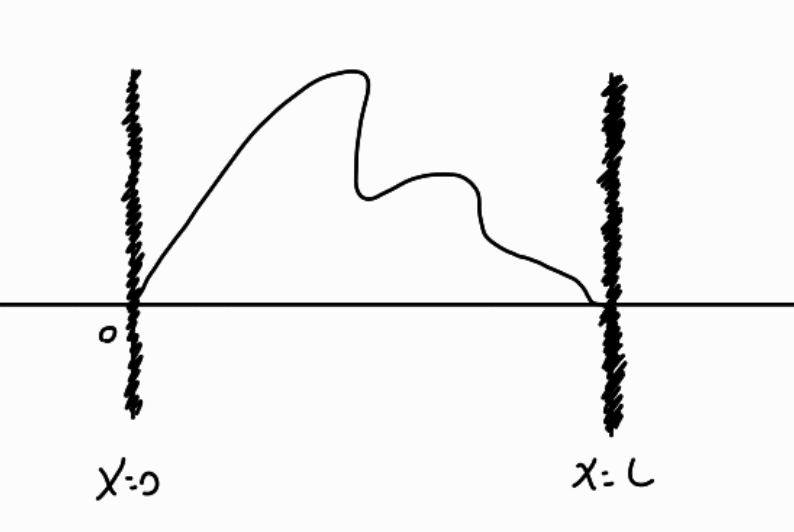
\includegraphics[scale=0.5]{fig/sin}
\end{figure}
Notar que para $\r(x,t=0)$, con $0<x<L$ \textit{arbitrario} puedo descomponer $\r(x,t=0)$ en serie de Fourier 
\begin{equation}
  \r(x,t=0)=\sum_{n=1}^\infty A_n(t=0)\sin\left(\frac{n\p x}{L}\right)
\end{equation}
y la solución está dada por
\begin{equation}
 \boxed{ A_n(t)=A_n(t=0)\exp\left[-D\left(\frac{n \p }{L}\right)^2t\right]}
\end{equation}

\subsection{Modelo de Ising en $D=1$}
El modelo de Ising está descrito por el siguiene Hamiltoniano
\begin{equation}
 \boxed{ H=-J\sum_{v.c}\s_i\s_j-\m B\sum_i\s_i},\qquad \s_i=\pm1 
\end{equation}
donde $v.c$ denota vecinos cercanos, $J$ es la constante de acoplamiento y $\m B$ es la energía magnética del spin en presencia de un campo externo en la dirección $z$ positivo.

Aproxima las interacciones en un sistema formado por una red de spines, donde por simplicidad solo consideramos la posibilidad de spin up y spin down.

\begin{ej}
	Si $\s_1=1$ y $\s_2=-1$ la contribución al Hamiltoniano será
	\begin{align}
  H&=-J(1)(-1)-\m B(1)-\m B(-1)\\
  &=J
\end{align}
\end{ej}

\begin{ej}
	Si Si $\s_1=1$ y $\s_2=1$ ,
	luego,
	\begin{equation}
  H=-J-2\m B
\end{equation}
\end{ej}

Consideremos $B=0$ y $D=1$, el ground-state correspode a todos los spines alineados hacia arriba, mientras que el caso de máxima energía conrresponde a todos alineados hacia arriba.



































